% !TeX root = ../latex-curto.tex
% !TeX encoding = utf8

\part{Conceitos básicos}

\section{Começando}

\begin{frame}
  \frametitle{Como funciona o \LaTeX}

  \begin{block}{Objetivo}
    Escrever \purple{documentos}, \textit{a priori} para impressão.
  \end{block}

  %\pause

  \bigskip

  MAS pode-se fazer ...

  \begin{itemize}
  \item \green{PDF com links}, no computador
  \item \blue{Apresentações em PDF} --- como essa!
  \end{itemize}

\end{frame}

\begin{frame}

  \frametitle{Como funciona o \LaTeX}


  \begin{description}
  \item[Edição de texto] usando \purple{EDITOR} apropriado\\
    escreve-se \green{\texttt{\textit{arquivo}.tex}} que descreve o documento

\bigskip
	
    %\pause

  \item[Compilação] \purple{``roda-se''} o programa \LaTeX{} (ou equivalente)
    \begin{itemize}
    \item em geral, de dentro do editor
    \end{itemize}

\bigskip
%\pause

  \item[Visualização] é gerado arquivo 
    \green{\texttt{pdf}}  (ou outros)\\
    para \purple{visualização} ou \cyan{impressão}


  \end{description}


%   \begin{itemize}

%   \item escreve-se um arquivo \texttt{\textit{arquivo}.tex}\\
%     em que se descreve o documento na linguagem \LaTeX

%     \begin{itemize}
%     \item \blue{EDITOR} apropriado é recomendável\\ --- exemplos:
%        TeXnicCenter, Winedt, TeXmaker, etc.
%     \end{itemize}

% %\pause

%   \item roda-se o programa \LaTeX{} (ou equivalente) e ``amigos''



% %\pause

%   \item é gerado arquivo para \emph{visualização} ou \emph{impressão}\\
%     (\texttt{pdf}, \texttt{ps} ou \texttt{dvi})

%   \end{itemize}

\end{frame}


\begin{frame}
 \frametitle{Prós e contras}

  %\uncover<1>

  \begin{alertblock}{Contras...}
    \begin{itemize}\medskip
    \item Não se vê o resultado enquanto se digita\\
      (como M\$ Word)\medskip
    \item Demora-se um pouco para aprender\medskip
    \end{itemize}
  \end{alertblock}

\end{frame}

\begin{frame}
 \frametitle{Prós e contras}

   MAS (uma vez aprendido) ...



   \begin{block}{Prós... que compensam}
     \begin{itemize}\medskip

     \item \LaTeX{} é mais \green{fácil} \smiley{}\\
       (fórmulas, referências, citações, sumário, etc.)\medskip

     \item Resultado \purple{bonito} e \blue{profissional}\medskip

     \item \purple{Gratuito} e disponível para todos os sistemas\medskip

     \end{itemize}
   \end{block}

\end{frame}


\section{Instalação}

\begin{frame}
  \frametitle{Instalação}

  \begin{block}{Windows: Mik\TeX $\quad\to$ www.miktex.org}
    \show\description
    \begin{description}
    \item[\purple{Versão básica (Basic Mik\TeX\ Installer)}] \ 
      \begin{itemize}
      \item pequena ($\approx$300Mb)
      \item Precisa de internet: instala pacotes conforme são usados
      \end{itemize}
    \item[\blue{Versão completa (Mik\TeX\ Net Installer)}] \ 
      \begin{itemize}
      \item $\approx 4Gb$
      \item 1º) Download (complete) $\to$ 2º) Install
      \item Funciona sem internet
      \end{itemize}
    \item[\green{Versão Portátil (Mik\TeX\ Portable)}] \ 
      \begin{itemize}
      \item Roda direto do pendrive, não precisa instalar
      \item Precisa de internet: instala pacotes conforme são usados
      \end{itemize}

    \end{description}
  \end{block}
  
\end{frame}

\begin{frame}
  \frametitle{Instalação}

  \begin{block}{Mac: Mac\TeX}
    \begin{itemize}
    \item Versão completa e fácil de instalar
    \end{itemize}
  \end{block}
  
  \begin{block}{Linux: \TeX live}
    \begin{itemize}
    \item Oferecida entre os programas disponíveis
    \end{itemize}
  \end{block}

  \begin{block}{Online, sem instalação}
    \begin{description}
    \item[\purple{\textsc{ShareLaTeX}}]\
      \begin{itemize}
      \item \url{www.sharelatex.com}
      \item Gratuito para uso pessoal
      \end{itemize}
    \end{description}
  \end{block}


\end{frame}


\begin{frame}
  \frametitle{Editor padrão: TeXWorks}
  
  \centering
  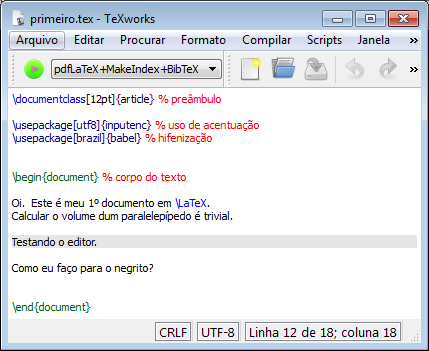
\includegraphics[scale=0.5]{./imagens/texworks-janela.png}

\end{frame}

\begin{frame}
  \frametitle{Editor padrão: TeXWorks}

  \begin{block}{TeXWorks}
    \begin{itemize}
    \item Já vem instalado quando instala-se o Mik\TeX
    \item Iterface funcional\\
      só o \blue{botão de
      rodar} 
\includegraphics[height=0.6\baselineskip]{./imagens/botao-latex.png}\ 
      e o \purple{menu de programas}\medskip

        \centerline{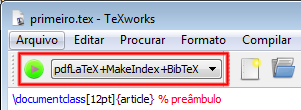
\includegraphics[scale=0.5]{./imagens/texworks-painel.png}}
      \item Visualizador de PDF com \purple{busca \LaTeX\ 
        $\leftrightarrow$ PDF}
    \end{itemize}
  \end{block}


\end{frame}




\section{A linguagem \LaTeX}

\begin{frame}

  \begin{block}{A linguagem \LaTeX}
    \begin{itemize}
      \medskip
    \item Essencialmente é \green{texto} ... \medskip %\pause
    \item ... organizado com \purple{comandos} e \blue{ambientes} \LaTeX.
      \medskip
    \end{itemize}
  \end{block}

\end{frame}

\begin{frame}
\frametitle{Básico de comandos em \LaTeX}


  \begin{block}{Comandos}

    \texttt{\purple{\bfseries{\bs}\textit{comando}}}\smallskip

    ou\smallskip

    \texttt{\purple{\bfseries{\bs}\textit{comando}}$\underbrace{\text{\red{[\textit{opcional}]}\brown{\ac\textit{arg$1$}\fc}}
        \cdots \text{\brown{\ac \textit{arg$n$}\fc}}}_{\text{parâmetros}}$}

  \end{block}

Exemplos

\begin{itemize}
\item \texttt{\purple{\string\alpha}} \quad ($\to\alpha$)
\item \texttt{\purple{\bs sqrt}\brown{\ac{}2\fc}} \quad
  ($\to\sqrt{2}$)
\item \texttt{\purple{\bs sqrt}\red{[3]}\brown{\ac{}2\fc}} \quad
  ($\to\sqrt[3]{2}$)
\end{itemize}

\end{frame}


\begin{frame}
\frametitle{Comandos em \LaTeX}

  \begin{block}{Agrupando com chaves \texttt{\ac{}...\fc{}}}

    \begin{itemize}\smallskip
    \item \purple{\texttt{Texto}} $\to$ 5 caracteres: T, e, x, t, o\smallskip
    \item \green{\texttt{\ac{}Texto\fc{}}} $\to$ 1 grupo = 1 coisa
    \end{itemize}

  \end{block}

%\pause

  \begin{exemplo}

    \begin{itemize}\smallskip
      \item  \purple{\texttt{\string\textbf}} \brown{\texttt{arg1}}\\
      $\to$ escreve \brown{\texttt{arg1}} em \textbf{negrito}\\
      \qquad \gray{(bf = bold face = negrito)}\bigskip

%\pause

    \item \blue{\texttt{\string\textbf\ Texto}} $\to$ \textbf Texto
      \quad \gray{(arg1 = T)}\smallskip
    \item \blue{\texttt{\string\textbf\ac{}Texto\fc{}}} $\to$
      \textbf{Texto} \quad \gray{(arg1 = Texto)}
      \smallskip
    \end{itemize}

  \end{exemplo}
\end{frame}



\begin{frame}
\frametitle{Ambientes}


  \begin{block}{Ambiente}\medskip

    \begin{itemize}
    \item Outro conceito importante é o \purple{ambiente}\\
      $\to$ delimita uma \green{região} do texto para um certo
      fim\medskip

%      \pause
 %   \item
      \texttt{\purple{\string\begin}\brown{\ac{}\textit{nome-do-ambiente}\fc{}}}

        \quad Texto dentro do ambiente

        \texttt{\purple{\string\end}\brown{\ac{}\textit{nome-do-ambiente}\fc{}}}
      \medskip
    \end{itemize}


  \end{block}


\medskip

%\pause

\begin{exemplos}
  
  % \begin{minipage}[t]{3cm}
  %   \begin{itemize}
  %   \item \texttt{document}
  %   \item \texttt{equation}
  %   \item \texttt{abstract}
  %   \end{itemize}
  % \end{minipage}
  % \qquad
  \begin{minipage}[t]{3cm}
    \texttt{\purple{\string\begin\brown{\ac{}equation\fc{}}}\\
        \mbox{}\ \ x\textasciicircum{}2\ -\ 1\ =\ 0\\
        \purple{\string\end}\brown{\ac{}equation\fc{}}}
  \end{minipage}
  \hfill
    \begin{minipage}[t]{6.5cm}
      \begin{equation}
        x^2-1=0       
      \end{equation}
    \end{minipage}
  \end{exemplos}

\end{frame}

\begin{frame}
 \frametitle{Estrutura básica: preâmbulo e corpo do texto}

%Exemplo de um documento simples: %(\texttt{primeiro.tex})

  \begin{code}\small
    % \documentclass[12pt]{article}     % preâmbulo
    %
    % \usepackage[latin1]{inputenc}     % uso de acentuação
    % \usepackage[brazil]{babel}        % hifenização
    %
    %
    % \begin{document}                  % corpo do texto
    %
    % Oi.  Este é meu 1º documento em \LaTeX.
    %
    % \end{document}
    \purple{\string\documentclass}\green{[12pt]\ac{}article\fc{}}\\%\ \ \ \ \ \gray{\textit{\pc{}\ preâmbulo}}a\\
\ \\
    \gray{\textit{\pc\ aqui declaram-se\ os\ pacotes\ usados,}}\ \ \
    \gray{%
      \raisebox{0cm}[0cm][0cm]{\makebox[0pt][r]{$\left.\rule{0pt}{1.1cm}\right\}$}} preâmbulo}\\
    \gray{\textit{\pc\ definem-se comandos e formatações}}\\ \ \\

%    \string\usepackage[latin1]\ac{}inputenc\fc{}a\\
%    \string\usepackage[brazil]\ac{}babel\fc{}a\\%\ \ \ \ \ \ \ \ \gray{\textit{\pc{}\ hifenização}}a\\
    \blue{\string\begin\ac{}document\fc{}}\\
\ \\
    O texto do documento vem aqui.\ \ \ \ \ \ \ \ \ \     \gray{%
      \raisebox{0cm}[0cm][0cm]{\makebox[0pt][r]{$\left.\rule{0pt}{1.1cm}\right\}$}}
      \makebox[0cm][l]{corpo do texto}}\\
\ \\
    \blue{\string\end\ac{}document\fc{}}
  \end{code}

\end{frame}


\begin{frame}
\frametitle{Classes dos documentos}

Para cada tipo, \purple{classes de documento}


\begin{block}{}\centering
  \texttt{\large\purple{\string\documentclass}\green{[$\underbrace{\text{a4paper,12pt}}_{\text{opções}}$]}\blue{\ac{}$\underbrace{\text{report}}_{\text{classe}}$\fc{}}}\par
\end{block}

\begin{block}{Classes comuns}
  \begin{itemize}
  \item \purple{\texttt{report}}, \blue{\texttt{book}}, \red{\texttt{amsbook}} $\to$ livros
  \item \blue{\texttt{article}}, \purple{\texttt{amsart}} $\to$ artigos
  \item \green{\texttt{beamer}} (como neste slide) $\to$ apresentações
  \end{itemize}
\end{block}


\end{frame}

\begin{frame}
\frametitle{Estendendo \LaTeX: pacotes}

  \begin{block}{Pacotes}
    \texttt{\purple{\string\usepackage}\green{[\textit{opções}]}\blue{\ac{}\textit{pacote}\fc{}}}
  \end{block}


\begin{block}{}
  \begin{description}
  \item[babel] hifenação e localização\qquad \gray{(opção \green{brazil})}
  \item[inputenc] acentuação\qquad \gray{(opção \green{utf8} no nosso
      caso, \green{latin1})}
%  \item[ae] boas fontes no pdf com fonte Computer Modern\qquad  \gray{(ae = almost european)}
  \item[geometry] dimensões de margens, etc.
  \item[amsmath, amssymb] %(inclua-os!) \\
    ambientes de fórmulas, símbolos ($\nexists \therefore \mathbb{R}$) etc.
  \item[graphicx] inclusão de imagens (jpg, png, pdf).
  \item[tikz] desenho de figuras
    \tikz[scale=0.15,rotate=90] \draw
    (0:1)--(2*72:1)--(4*72:1)--(6*72:1)--(8*72:1)--cycle;
    \tikz[scale=0.15] \draw (0,0) ellipse[x radius=1.7,y radius=1];
    
\begin{tikzpicture}[scale=0.32]
      \draw[gray]  (72:1) arc(72:45:1) (0:1) ++(135:1) arc(135:110:1);
      \draw (0,0) -- (0:1) -- (60:1) -- cycle;      
    \end{tikzpicture}
  \item[bm] (\textbf{b}old \textbf{m}ath) fórmulas em negrito $\bm{e^{i\pi}+1 = 0}$.
  \item[multicol] Texto em várias colunas.
  \end{description}
\end{block}

\centering

  \gray{e muitíssimos outros (centenas).}

\end{frame}

%\section{Um pouco mais do básico de \LaTeX}

% \begin{frame}
% \frametitle{Caracteres especiais}

% Alguns caracteres são usados na linguagem (``reservados'')\bigskip

% \small
% \begin{tabular}{l|l|l}
%   % \purple{\texttt{\bs}} & início de comando & \blue{\texttt{\footnotesize\string\textbackslash}}  \gray{\footnotesize(\texttt{\string\\} = nova linha)} \\
%   \purple{\texttt{\dolar}} & muda modo matemático & \blue{\texttt{\string\$}} \\
%   \purple{\texttt{\et}} & tabulador & \blue{\texttt{\string\&{}}} \\
%   \purple{\texttt{\pc}} & comentário & \blue{\texttt{\string\%}} \\
%   \purple{\texttt{\num}}& def.\ comando & \blue{\texttt{\string\#}} \\
%   \purple{\texttt{\string~}} & espaço inquebrável &
%   % \blue{\texttt{\string\~\ac\fc}}\quad \gray{\footnotesize(acento til em nada)}\\
%   % \purple{\texttt{\string|}} & linhas vert. em tabelas &
%   % \blue{\texttt{\string\textbar}} \\
%   % \purple{\texttt{\string_}} & índice subescrito & \blue{\texttt{\string\_}} \\
%   % \purple{\texttt{\^{}}} & índice superscrito &
%   % \blue{\texttt{\string\^\ac\fc}} \quad \gray{\footnotesize(acento circunflexo em nada)}\\
%   % \purple{\texttt{\ac{} \fc}} & delimitador de grupos & \blue{\texttt{\string\{\
%   %    \string\}}}\\
%   %  \purple{\texttt{`` ''}} & aspas & \blue{\texttt{\grave\grave{} \aspa\aspa}}
%   %  \gray{(obs: \texttt{\aspa} $\neq$ \'{})}\\
%   %  \purple{\texttt{\maior{} \menor}} & tabulação & \blue{\texttt{\string\textgreater{} \string\textless}}
% \end{tabular}

% \end{frame}


\begin{frame}
  \frametitle{Texto e fórmulas}
  
  \begin{itemize}
  \item Digite \green{texto} normalmente.
  \item Novo parágrafo $\to$ deixe uma linha em branco.
  \item \purple{Fórmulas no parágrafo} $\to$ entre \purple{\texttt{\dolar}} e \purple{\texttt{\dolar}}: \quad
    \texttt{\purple{\dolar}\blue{\string\sqrt\ac{}x\fc{}}\purple{\dolar}}
    $\to \sqrt{x}$
  \item \blue{Fórmulas em destaque} $\to$ entre \blue{\texttt{\string\[}} e
      \blue{\texttt{\string\]}}\dots\ ou outros
  \end{itemize}

  \begin{exemplo}\small
        \texttt{Seja \purple{\dolar{}}\blue{f(x)}\purple{\dolar{}} a função dada por\\
          \purple{\string\[}\\
              \ \ \blue{f(x)\ =\ \string\frac\ac{}x\textasciicircum{}2\ +\ 1\fc{}\ac{}\string\cos\ x\fc{}}\\
              \purple{\string\]}}

        \bigskip\hrule\bigskip

        Seja $f(x)$ a função dada por
        \[
          f(x) = \frac{x^2 + 1}{\cos x}
        \]
  \end{exemplo}

\end{frame}




\begin{frame}
\frametitle{Acentos}

    \begin{block}{Escreva acentos normalmente}\medskip

      Use pacote \purple{inputenc} para acentuar normalmente\medskip

      \centering \texttt{\purple{\string\usepackage}\red{[utf8]}\blue{\ac{}inputenc\fc{}}}\medskip\par
    \end{block}

    \begin{alertblock}{Use a opção certa}
      \texttt{\purple{utf8}} -- codificação UTF-8\\
      \texttt{\purple{latin1}} -- codificação ISO 8859-1 = Latin-1      
    \end{alertblock}

  %   \begin{alertblock}{Acentos à moda antiga \hfill (não recomendado)}

  %     \begin{itemize}
  %     \item ilegível
  %     \item impede corretores ortográficos
  %     \end{itemize}

  %     \centering
  %   \begin{tabular}{p{4cm}p{2.5cm}}
  %     \green{fonte} & \green{saída} \\
  %     \blue{\texttt{\string\'orf\string\~ao}} & \'orf\~ao \\
  %     \blue{\texttt{ling\string\"ui\string\c\ac{}c\fc{}a}} & ling\"ui\c ca \\
  %     \blue{\texttt{ci\string\^encia}} & ci\^encia \\
  %   \end{tabular}
  % \end{alertblock}

\end{frame}


%%% Local Variables: 
%%% mode: latex
%%% TeX-master: "../latex-curto"
%%% End: 
